\documentclass[acmsmall,screen,nonacm]{acmart}

%% Course manuscript; ACM copyright block suppressed.
\settopmatter{printacmref=false}
\renewcommand\footnotetextcopyrightpermission[1]{}
\setcopyright{none}
\acmConference{}{}{}
\acmYear{2026}
\copyrightyear{2026}
\pagestyle{plain}

\usepackage{graphicx}
\usepackage{amsmath}
\usepackage{booktabs}
\usepackage{array}
\newcolumntype{L}[1]{>{\raggedright\arraybackslash}p{#1}}

\title{Effect of Citation-Count Features on Lower-Citation Recall in AI Literature Curation}

\author{Aditya Chaudhary}
\affiliation{%
  \institution{Indian Institute of Information Technology, Allahabad}
  \country{India}
}

\begin{abstract}
Scholarly search and screening tools often use citation counts as a ranking signal. This study asks
whether adding an explicit citation-count feature to a transparent relevance ranker changes how many
relevant but rarely cited papers reach the top of a screening queue. We collected a quota-stratified
candidate pool of 2,790 OpenAlex records (2015--2025) through English keyword queries, topic filters
and the citation neighbourhoods of five seed papers, audited its metadata, and screened 2,763 records
against a written relevance rubric. An AI assistant applied the rubric to all records first; the author
then reviewed the 458 records that were relevant, uncertain or close to the boundary, changing 15
decisions. The remaining 2,305 clearly off-topic records keep the AI screener's label. Of 2,754 decided
records, 64 (2.3\%) were relevant, and only 7 of these fell in the lower half of the age-adjusted citation
distribution. The pre-registered dataset gate, which requires at least 20
relevant records in each citation group of the test split, therefore failed, and all results are
exploratory. Two Logistic Regression rankers that differed only in a standardised
$\log(1+\text{citations})$ feature were compared. On the frozen single split the primary metric was not
estimable (one relevant lower-citation test record). In a cross-fitted analysis over the same five
grouped folds, the citation-blind ranker placed all 7 lower-citation relevant records in the top 20\% of
its fold, against 3 of 7 for the citation-aware ranker (paired difference 0.57; 95\% cluster-bootstrap
interval 0.14 to 1.00), and overall Recall@20\% fell from 0.984 to 0.891. The direction is consistent with
the concern that citation features push relevant, rarely cited work down the queue, but the evidence
rests on seven records and a pool whose relevant records came mostly from citation neighbourhoods. The contribution is a reproducible, fail-closed evaluation pipeline and a worked
demonstration of why group-conditional recall needs much larger labelled pools.
\end{abstract}

\begin{CCSXML}
<ccs2012>
<concept>
<concept_id>10002951.10003317.10003338.10003341</concept_id>
<concept_desc>Information systems~Information retrieval</concept_desc>
<concept_significance>500</concept_significance>
</concept>
</ccs2012>
\end{CCSXML}
\ccsdesc[500]{Information systems~Information retrieval}

\keywords{citation bias, recall, literature screening, systematic review automation, feature ablation, OpenAlex}

\begin{document}
\maketitle
\setlength{\emergencystretch}{2em}

\section{Introduction}
\label{sec:intro}

Many tools that help researchers find and screen literature rank records partly by how often they have
been cited. Google Scholar has been shown to weight citation counts heavily in its ranking
\cite{beel2009citation}, and scholarly recommenders are known to over-expose popular items
\cite{farber2023biases,klimashevskaia2024survey}. Citation counts are themselves shaped by cumulative
advantage \cite{merton1968matthew} and by factors unrelated to a study's content
\cite{duyx2017scientific,lund2025predictors}. If a ranker learns that relevant papers tend to be highly
cited, it may rank relevant but rarely cited papers lower, and in a prioritised screening workflow those
papers are the ones most likely to be left unread when screening stops \cite{callaghan2020stopping}.

Evaluations of screening tools usually report recall for a whole collection
\cite{przybyla2018prioritising,vandeschoot2021asreview,aigner2026comparing}. Whether that recall is
lower for less-cited papers is rarely measured. This study isolates one mechanism: it trains two
otherwise identical rankers, one with and one without an explicit citation-count feature, and compares
how many relevant lower-citation records each places in the top $K$ of a held-out queue.

The study does not estimate how any commercial search engine behaves, and it does not test language
effects confirmatorily. It reports what a small, carefully audited pool can and cannot show about the question. Because the pre-registered data gate failed, all results are
exploratory.

\section{Research Questions}
\label{sec:rq}

\begin{description}
\item[RQ1 (primary).] In a fixed candidate pool, does adding a $\log(1+\text{citations})$ feature to a
TF--IDF Logistic Regression ranker change Recall@K for relevant lower-citation records? The contrast is
$\Delta_{\text{low}} = \text{Recall}_{\text{low}}@K(A) - \text{Recall}_{\text{low}}@K(B)$, where $A$ is
citation-blind and $B$ citation-aware; a positive value favours $A$.
\item[RQ2.] Does the citation feature change the gap between higher- and lower-citation recall?
\item[RQ3 (conditional).] Do English and non-English metadata-language records differ? This was to be
analysed only if publication languages were verified and each group had at least 20 relevant test
records.
\end{description}

The frozen protocol made no prediction about the direction of $\Delta_{\text{low}}$.

\section{Data}
\label{sec:data}

\subsection{Candidate pool}

The pool was collected from the OpenAlex API \cite{priem2022openalex} on 30 October 2026 (citation
snapshot date). Three kinds of route were used, each restricted to records with abstracts published
2015--2025: eight English keyword queries (for example \emph{automated literature screening},
\emph{scholarly information retrieval}, \emph{active learning title abstract screening}) and four OpenAlex
topic filters, each sampled at 20 records per publication year with OpenAlex's seeded random sampling;
and the incoming citers and outgoing references of five seed papers on screening, citation searching,
scholarly recommender bias and language bias in retrieval. No route was sorted by citation count. After
deduplication by OpenAlex identifier the pool held 2,790 records, with 247--262 records in each year.
The pool is a quota-stratified sample of query frames, not a census, so all recall values are relative to
it.

\subsection{Metadata audit}

Before screening, 27 records were withheld: 6 whole-issue records verified on publisher pages, 13
records with missing titles that could not be repaired from source, and 8 administrative records
(retraction flags, retraction notices, errata and a superseded version). Duplicate and version
relationships were reviewed manually and recorded in a \texttt{split\_group\_id}; one two-version group
was found. The OpenAlex language field is inferred from metadata and can be wrong
\cite{cespedes2025openalex}; it is called \emph{metadata language} here because no publication language
was verified.

\subsection{Relevance screening and label provenance}

Records were screened on title and abstract against Annotation Rubric v2. A record is relevant only if it
studies, develops or evaluates a computational or AI method whose target task is discovering, ranking,
recommending, screening or selecting scholarly literature. Reviews of AI in an application domain,
downstream extraction from study content, and bibliometric analyses are not relevant.

\textbf{Screening procedure and label provenance.} Screening ran in two stages. First, an AI assistant
(Claude, Anthropic) applied Rubric v2 to all 2,763 records, recording a label, a coded rationale and a
confidence level for each. A seeded random 20\% of its decisions (550 records, seed 20261030) was
re-screened by the same assistant without access to its first-pass labels: 549 of 550 agreed. Second, the
author reviewed every record that the first pass marked relevant or uncertain (72), every negative it had
examined closely (53), and every remaining negative containing curation-related terms (333), 458 records in
all, assigning their own label, rationale and confidence. Author and AI agreed on 443 of the 458 records
(Cohen's $\kappa = 0.88$). The author changed 15 decisions: one uncertain record became relevant, four
relevant and two uncertain records became not relevant, and eight became uncertain. Records the author
marked uncertain (9) are excluded from modelling. The other 2,305 records, which the first pass judged
clearly unrelated to scholarly-literature curation, were not individually reviewed by the author and keep
the AI label; their status is recorded as \texttt{ai\_provisional} in the data files.

Table~\ref{tab:screening} summarises the outcome. Of 2,754 decided records, 64 were relevant. They cover
machine-assisted screening, scholarly search and discovery systems, citation-based searching, paper
recommendation and review automation. Relevance was very unevenly distributed across routes: 46 relevant
records (72\%) were reached through citation neighbourhoods, which contributed only 145 decided records,
whereas the 1,740 keyword-route records contained 10 relevant records (0.6\%).

\begin{table}[t]
\caption{Screening outcome by retrieval route (final labels). Records reached by several routes are
counted in each.}
\label{tab:screening}
\small
\begin{tabular}{L{4.2cm}rrr}
\toprule
Route & Decided records & Relevant & Relevant (\%) \\
\midrule
Keyword search (8 queries) & 1,740 & 10 & 0.6 \\
Topic filter (4 topics) & 865 & 5 & 0.6 \\
Citation neighbourhood (5 seeds) & 145 & 46 & 31.7 \\
Seed papers & 5 & 4 & 80.0 \\
\midrule
All decided records & 2,754 & 64 & 2.3 \\
\bottomrule
\end{tabular}
\end{table}

\section{Methods}
\label{sec:methods}

\subsection{Rankers}

Both conditions use the same scikit-learn pipeline \cite{pedregosa2011scikit}: TF--IDF features of title
and abstract (unigrams and bigrams, minimum document frequency 2, sublinear term frequency) plus
standardised publication year, and Logistic Regression ($C = 1$, balanced class weights, liblinear
solver, random state 20261030). Condition B adds one standardised feature,
$\log(1 + \text{citations})$, with scaling fitted on training data only. Nothing else differs. Each
condition ranks the test records by predicted probability, breaking ties by OpenAlex identifier.

\subsection{Citation groups and metrics}

Citations are adjusted for exposure time as a citation rate, citations divided by
$\max(1, 2026 - \text{year} + 1)$. Records at or below the pool median rate (0.408 citations per year)
form the lower-citation group. The group definition is not a field-normalised impact measure. The
primary metric is lower-citation Recall@K with $K = \lceil 0.20 N_{\text{test}} \rceil$: the share of
relevant lower-citation test records ranked in the top $K$. Overall Recall@K, Precision@K and
higher-citation Recall@K are secondary; $K$ at 10\% and 30\% are pre-specified sensitivity analyses.

\subsection{Frozen design and dataset gate}

The frozen protocol uses five-fold \texttt{StratifiedGroupKFold} (seed 20261030) with fold 0 as test,
fold 1 as validation and folds 2--4 as training, so that version groups never cross partitions. Before
any model is fitted, the test fold must contain at least 20 relevant lower-citation and 20 relevant
higher-citation records. The paired difference is bootstrapped by resampling \texttt{split\_group\_id}
clusters (2,000 replicates, seed 20261031). The protocol's success rule requires $\Delta_{\text{low}} > 0$,
a bootstrap lower bound above 0 and a Precision@K loss of no more than 0.05 for condition A.

\subsection{Amendment A3: exploratory analyses}

Amendment A3 was recorded before any model was fitted, once screening showed that the gate could not
pass. It specifies: (i) the gate is reported as failed; (ii) the frozen single-split comparison is still
run, labelled exploratory; and (iii) a cross-fitted analysis uses each of the same five folds once as the
test fold, training on the other four. Recall@K is computed within each fold and pooled across folds
(relevant records ranked in the top $K$ of their fold, divided by all relevant records), and the paired
difference is bootstrapped by resampling clusters within folds. After the frozen exploratory run returned
a degenerate result (Section~\ref{sec:frozen}), a reporting guard was added that marks the primary
estimate as not estimable when fewer than 10 relevant lower-citation test records are present; this is
disclosed in the amendment addendum and changes no estimate.

\section{Results}
\label{sec:results}

\subsection{Dataset gate}

The gate failed. Relevant records were concentrated among highly cited works: their median citation
count was 38, against 2 for non-relevant records, and only 7 of the 64 fell in the lower-citation group.
The frozen test fold contained 13 relevant records, 1 in the lower-citation group and 12 in the
higher-citation group. Training data contained 38 relevant records, of which 5 were lower-citation.

\subsection{Frozen single split (exploratory)}
\label{sec:frozen}

The citation-blind ranker placed all 13 relevant test records in the top $K = 111$ of 551 records; the
citation-aware ranker placed 10, missing two higher-citation records and the single lower-citation record, so $\Delta_{\text{low}} = 1$ and the bootstrap interval was the degenerate $[1, 1]$.
With one record in the denominator this comparison carries no information beyond that single case and is
reported as not estimable. Precision@K was 0.117 for condition A and 0.090 for condition B.

\subsection{Cross-fitted analysis (exploratory)}

Table~\ref{tab:crossfit} and Figure~\ref{fig:recall} give pooled results over the five folds. The
citation-blind ranker placed all 7 lower-citation relevant records in the top 20\% of their test folds;
the citation-aware ranker placed 3. The paired difference in lower-citation Recall@20\% was 0.57 (95\%
cluster-bootstrap interval 0.14 to 1.00). Higher-citation recall changed less (0.982 against 0.947;
difference 0.035, interval 0.000 to 0.088). Overall recall fell from 0.984 to 0.891 (difference 0.094,
interval 0.019 to 0.167), and Precision@20\% fell slightly, from 0.114 to 0.103. The citation feature
therefore did not buy any gain in this pool; it lowered both overall and lower-citation recall.

\begin{table}[t]
\caption{Cross-fitted pooled results (five folds, final labels, exploratory). Counts are relevant records in
the top $K$ of their fold over relevant records.}
\label{tab:crossfit}
\small
\begin{tabular}{lrrrr}
\toprule
 & \multicolumn{2}{c}{Citation-blind (A)} & \multicolumn{2}{c}{Citation-aware (B)} \\
\cmidrule(lr){2-3}\cmidrule(lr){4-5}
Group, $K$ & hits & recall & hits & recall \\
\midrule
Lower-citation, 20\% & 7/7 & 1.000 & 3/7 & 0.429 \\
Higher-citation, 20\% & 56/57 & 0.982 & 54/57 & 0.947 \\
All relevant, 20\% & 63/64 & 0.984 & 57/64 & 0.891 \\
\addlinespace
Lower-citation, 10\% & 7/7 & 1.000 & 1/7 & 0.143 \\
Lower-citation, 30\% & 7/7 & 1.000 & 6/7 & 0.857 \\
All relevant, 10\% & 63/64 & 0.984 & 52/64 & 0.812 \\
\bottomrule
\end{tabular}
\end{table}

\begin{figure}[t]
\centering
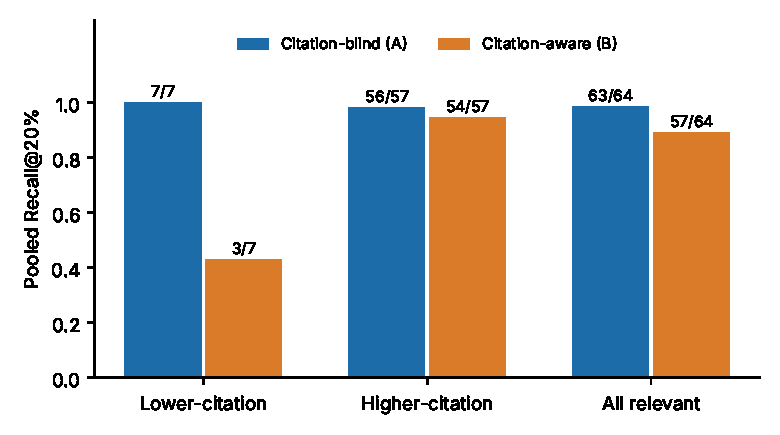
\includegraphics[width=0.68\linewidth]{fig_recall_by_group.pdf}
\caption{Pooled Recall@20\% by citation group in the cross-fitted analysis. Labels give relevant records
in the top $K$ over relevant records in the group.}
\label{fig:recall}
\end{figure}

The pre-specified sensitivity cutoffs show the same direction (Table~\ref{tab:crossfit}): at 10\% the
citation-aware ranker retrieved 1 of 7 lower-citation relevant records, and at 30\% it retrieved 6 of 7,
while the citation-blind ranker retrieved all 7 at every cutoff.

\subsection{Error analysis}

Figure~\ref{fig:rankshift} shows where the seven lower-citation relevant records were ranked within their
test folds. All had between 0 and 3 citations. Under the citation-blind ranker they sat at ranks 1 to 40;
under the citation-aware ranker four moved below the cutoff, to ranks between 126 and 280, and the other
three fell from ranks 1--20 to ranks 10--93. Two were published in 2025 and two in 2024, so they have had
little time to be cited; others are older papers that never attracted citations, for example a 2015 article
on using full-text citation networks to improve keyword labelling. The seven records are spread across all
five folds (three in one fold, one in each of the others). Among higher-citation relevant records, an
Indonesian-language thesis-search system was missed by both rankers (ranks 514 and 384), and two records
with six citations each, a library discovery-tool evaluation and a search system for the COVID-19 research
collection, were retrieved by the citation-blind ranker (ranks 38 and 34) but not by the citation-aware
ranker (ranks 120 and 117).

\begin{figure}[t]
\centering
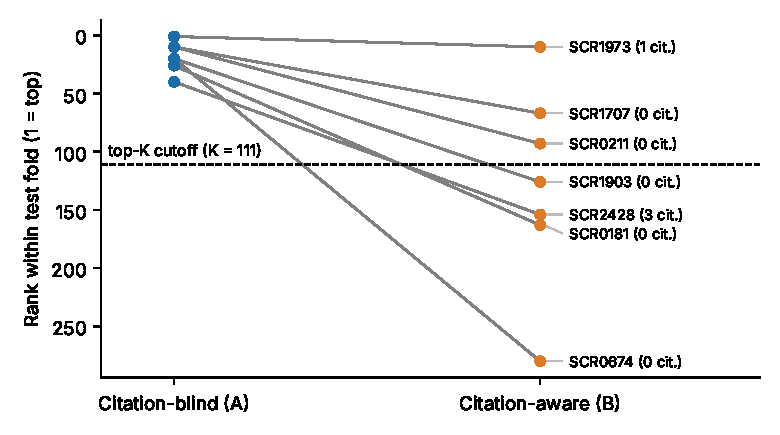
\includegraphics[width=0.68\linewidth]{fig_rank_shift_lower_citation.pdf}
\caption{Rank within test fold of the seven relevant lower-citation records under each ranker. Smaller
ranks are better; the dashed line marks the top-$K$ cutoff in a 551-record fold.}
\label{fig:rankshift}
\end{figure}

\subsection{Language}

Of the 64 relevant records, 61 had English metadata, and one each Spanish, Indonesian and Thai. No publication
language was verified. RQ3 cannot be addressed with these data.

\subsection{Resources}

Each ranker took about one second to fit and about 0.2 seconds to score a 551-record fold on a standard
CPU; the full cross-fitted analysis with 2,000 bootstrap replicates took about 30 seconds.

\section{Discussion}
\label{sec:discussion}

The cross-fitted result points the way the motivating concern predicts. When relevant records in the
training data are mostly highly cited, a citation feature becomes a proxy for relevance, and relevant
records that are rarely cited are pushed down the queue even when their text clearly matches the task. In
this pool the cost was not confined to the lower-citation group: overall recall also fell, because highly
cited but irrelevant records displaced relevant ones from the top $K$.

Three features of the data limit how far this can be taken. First, the comparison rests on seven records;
the within-fold bootstrap does not capture variation from model refitting or fold composition, so the
interval is likely too narrow. Second, the citation advantage of relevant records is largely an
artefact of collection. Seventy-two per cent of relevant records came from the citation neighbourhoods of
five seed papers, which are by construction connected to cited work; keyword routes with random sampling
returned mostly off-topic records. A pool built differently could show a very different citation profile
among relevant records, and the effect of the citation feature depends on that profile. Third, the 2,305 records the author did not review keep AI labels; a missed relevant record
among them could change the small lower-citation group materially, although these records contained no
curation-related terms.

The study therefore does not show that citation features harm lower-citation recall in AI literature
curation generally. It shows that, in one audited pool, the measurement is feasible, the direction is
consistent with the concern, and the denominators needed for a confirmatory test are far larger than this
pool provides: with relevant prevalence near 2.3\% and few relevant records in the lower-citation half, a
pool of several tens of thousands of screened records, or a collection design that oversamples
low-citation relevant records, would be needed to meet the frozen gate.

\section{Threats to Validity}
\label{sec:threats}

\textbf{Construct validity.} Relevance is defined narrowly by Rubric v2; a broader definition would change
prevalence and the citation profile of relevant records. The citation group is a pool-median split of an
age-adjusted rate, not field-normalised impact.

\textbf{Internal validity.} The two rankers differ in one feature only, so differences between them are
attributable to that feature within this pool. Labels were assigned by an AI screener and, for the 458
boundary and relevant records, reviewed by the author, who knew the study's question; citation counts were
not shown in the screening sheets.

\textbf{Statistical conclusion validity.} The lower-citation denominator is 7; the frozen gate failed;
the cross-fitted analysis was added by amendment; and a reporting guard was added after one output was
seen. All results are exploratory.

\textbf{External validity.} Results are relative to one OpenAlex pool, one snapshot date, English keyword
queries and one linear ranker. They say nothing direct about commercial search engines or modern neural
rankers.

\section{Reproducibility and Data Availability}

The collection, audit, screening-label, modelling and figure scripts, the frozen protocol, Amendments A2
and A3, the split manifests, out-of-fold predictions and all metric files are in the project repository.
An abstract-free metadata file and the final labels with their source (author or AI), rationales and
confidence are shareable; abstract text is kept private. OpenAlex data are released under CC0. All analyses run on a CPU in under a minute.
Re-running the two analysis commands on the final label file regenerates every number and figure in this
paper.

\begin{acks}
\textbf{Use of generative AI.} Generative AI (Claude, Anthropic) was used to assist with collection-code
development, metadata auditing, first-pass relevance screening of all 2,763 records, analysis code, and
drafting of this manuscript. The author reviewed the 458 relevant, uncertain and boundary records and made
the final decision on each; the remaining 2,305 records keep the AI first-pass label, as described in
Section~\ref{sec:data}. The author is responsible for the content.
\end{acks}

\bibliographystyle{ACM-Reference-Format}
\bibliography{references}

\end{document}
